\documentclass{article}

\usepackage[english]{babel}
\usepackage[a4paper]{geometry}
\usepackage{amsmath}
\usepackage{graphicx}
\usepackage[colorlinks=true, allcolors=blue]{hyperref}
\usepackage{pgf}
\usepackage{xcolor}

\title{Project Plan}
\author{Carl Schmidt-Svejstrup \& David Lindahl}

\begin{document}
\maketitle

\section*{Motivation}

The motivation behind this project is to develop a model that can assess speech quality in a descriptive string, similar to an audio expert. Demonstrating this as a proof of concept — that AI can evaluate audio in a comparable manner to a human expert — could significantly reduce the cost of large-scale data labeling.

Current SOTA audio-assessment datasets like NISQA contain MOS (Mean Opinion Scores) and other float values assessing quality; however, no current dataset exists that includes a text label describing the quality.\\
Filling this gap by creating such a dataset could potentially support research in noise-cancelling and hearing aid development.

\subsection*{Research Question}
\textit{Is it possible to train an audio LLM so that, given human audio as input, it outputs a high-quality audio assessment?}\\

Our hypothesis is that this is possible. Step one of this project will be to  re-implement the paper "Audio Large Language Models Can Be Descriptive Speech Quality Evaluator"\cite{chen2025audio}. From this standpoint, we will attempt to improve the model so that, instead of generating a "generic" string, it outputs something similar to an audio experts, in relation to GN's inquiry.\\

Answering this research question could contribute new knowledge by bridging the gap between numerical quality scores and expert-level descriptive evaluations.

\section*{Time plan}

In \autoref{fig:gantt} is our Gantt chart. We will update it dynamically, and you have access to our daily meetings and Gantt chart here:
\href{https://docs.google.com/document/d/1wSG3lSkr7cuSwWMX_2JGA9z1oDuxmNTsCSVygoZOwdk}{Project Gantt Chart and Meeting Notes}

\textbf{Risk analysis of possible delays:}
\begin{itemize}
    \item Re-implementing: The original paper does not include source code, but we do have access to their datasets and Swift scripts. Re-implementing in Python for more control over our experiment may be challenging and time-consuming.
    \item Analyzing results \& continuing development: Historically, we have experienced delays when finalizing code and moving forward instead of making additional changes. This typically occurs after analyzing results and identifying mistakes or potential improvements.
\end{itemize}

\begin{figure}
\centering
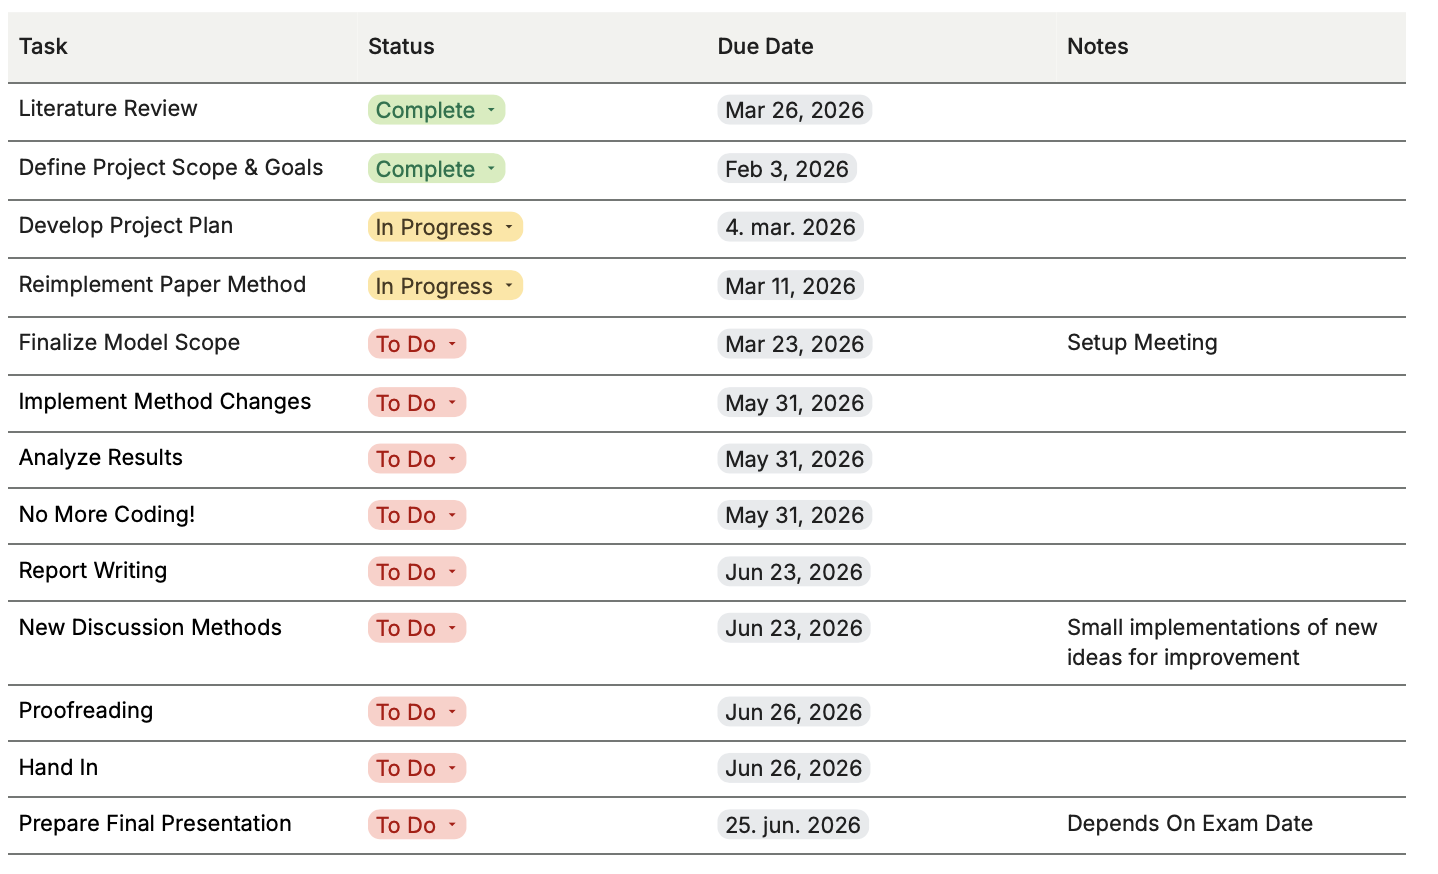
\includegraphics[width=0.8\textwidth]{../figures/Gantt-chart.png}
\caption{Gantt chart of the project plan.}\label{fig:gantt}
\end{figure}

\newpage

\nocite{*}
\bibliographystyle{plain}
\bibliography{bibliography}

\end{document}